% nota teorica

%%  incluir la informaci´on del microcontrolador(caracter´ısticas generales, diagrama de bloques, diagrama de pines y características eléctricas), perifricos utilizados (esto incluye descripción de registros e instrucciones seg´un aplique), componentes electrónicos complementarios; as´ı como también el diseño del circuito justificando los valores o función de los componentes electrónicos/digitales utilizados (debe incluir una lista de la cantidad de componentes y sus precios) e información de los conceptos fundamentales adicionales que se ven en clase

%informacion general mcu 
\subsection{Información general del STM32F429 Discovery kit}

El kit STM32F429 Discovery (modelo 32F429IDISCOVERY) está diseñado para facilitar el desarrollo de aplicaciones utilizando el microcontrolador STM32F429 de alto rendimiento, el cual está basado en el núcleo ARM Cortex-M4. Una de las características destacadas de este kit es la inclusión de la herramienta de depuración ST-LINK/V2 o ST-LINK/V2-B, una herramienta embebida que simplifica el proceso de depuración de aplicaciones, permitiendo a los desarrolladores identificar y corregir errores de software de manera eficiente. El kit viene equipado con una pantalla LCD TFT QVGA de 2,4 pulgadas que ofrece una interfaz visual para la salida de datos o para la creación de interfaces de usuario gráficas. En la figura \ref{STM}, se observa la pariencia física del microcontrolador STM32F429.

 \begin{figure}[H]
        \centering
        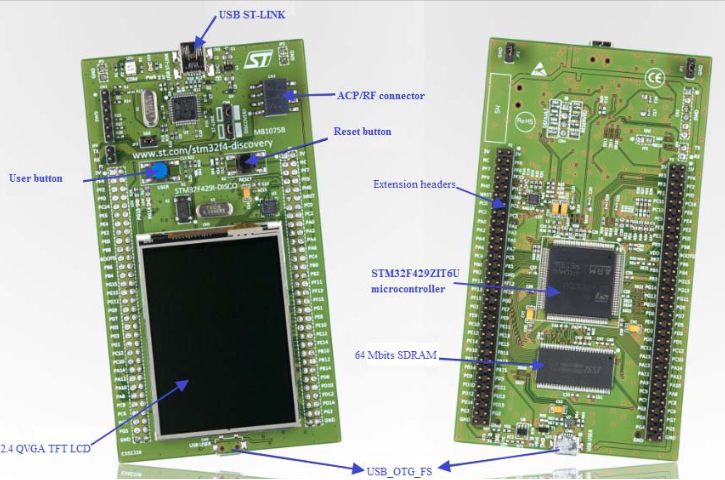
\includegraphics[width=1\linewidth]{fotos/STM.png}
        \caption{Microcontrolador STM32F429 \cite{STM}.}
        \label{STM}
    \end{figure}

    %caracteristicas 
    \subsubsection{Características}

    Se trabaja con un microcontrolador STM32F429ZIT6 con 2 MB de memoria Flash, 256 KB de RAM en un encapsulado LQFP144. La alimentación de la placa es a través del bus USB o desde una tensión de alimentación externa de 3 V o 5 V, como una batería. Para el almacenamiento y manejo de datos en aplicaciones que requieren alta capacidad, el kit incluye SDRAM externa de 64 Mbits. Cabe mencionar, que el MCU está basado en el núcleo RISC ARM Cortex M4-32-bit, el cual opera a 180MHz. \cite{STM} \\

    Este MCU tiene incorporado el sensor de movimiento L3GD20 y una pantalla TFT LCD, elementos de los cuales se hablará más adelante. Se tiene un conector USB OTG micro-AB, el cual facilita la comunicación con otros dispositivos y la implementación de funcionalidades USB On-The-Go (OTG), permitiendo al dispositivo actuar tanto como host como dispositivo USB. \cite{STM} \\

    La configuración del microcontrolador incluye seis LEDs distintivos, los cuales están diseñados para señalizar diferentes estados y funciones: 
    \begin{itemize}
        \item LD1: LED dual que alterna entre rojo y verde para indicar la comunicación USB, facilitando la identificación de la actividad de transmisión de datos. \cite{STM} 
        \item LD2: LED rojo que se ilumina para señalar que el dispositivo está encendido y funcionando a 3,3 V, proporcionando una confirmación visual inmediata del estado de energía. \cite{STM}
    \end{itemize}
    
    Se disponen de dos LEDs que son específicamente para el usuario: LD3, verde, y LD4, rojo, diseñados para dar una interfaz visual que puede ser personalizada según las necesidades del usuario, permitiendo una amplia gama de aplicaciones de señalización y feedback. Luego, están los otros dos LEDs dedicados a la función USB OTG (On-The-Go), LD5 (verde), que indica la presencia de VBUS, y LD6,(rojo), que se ilumina en casos de sobrecorriente (OC), alertando sobre posibles condiciones de fallo eléctrico. \cite{STM} \\
    
    Para la interacción con el dispositivo, se tienen dos pulsadores: uno destinado al uso general por parte del usuario, que permite la entrada manual para control o configuración, y otro para la función de reset, que facilita la recuperación rápida del sistema en caso de necesidad. 
    
    %diagrama de bloques 
    \subsubsection{Diagrama de bloques}
    Se muestra el diagrama de bloques obtenido de la hoja de datos del Discovery kit for STM32F429/439 lines \cite{STM2}:
    
    \begin{figure}[H]
        \centering
        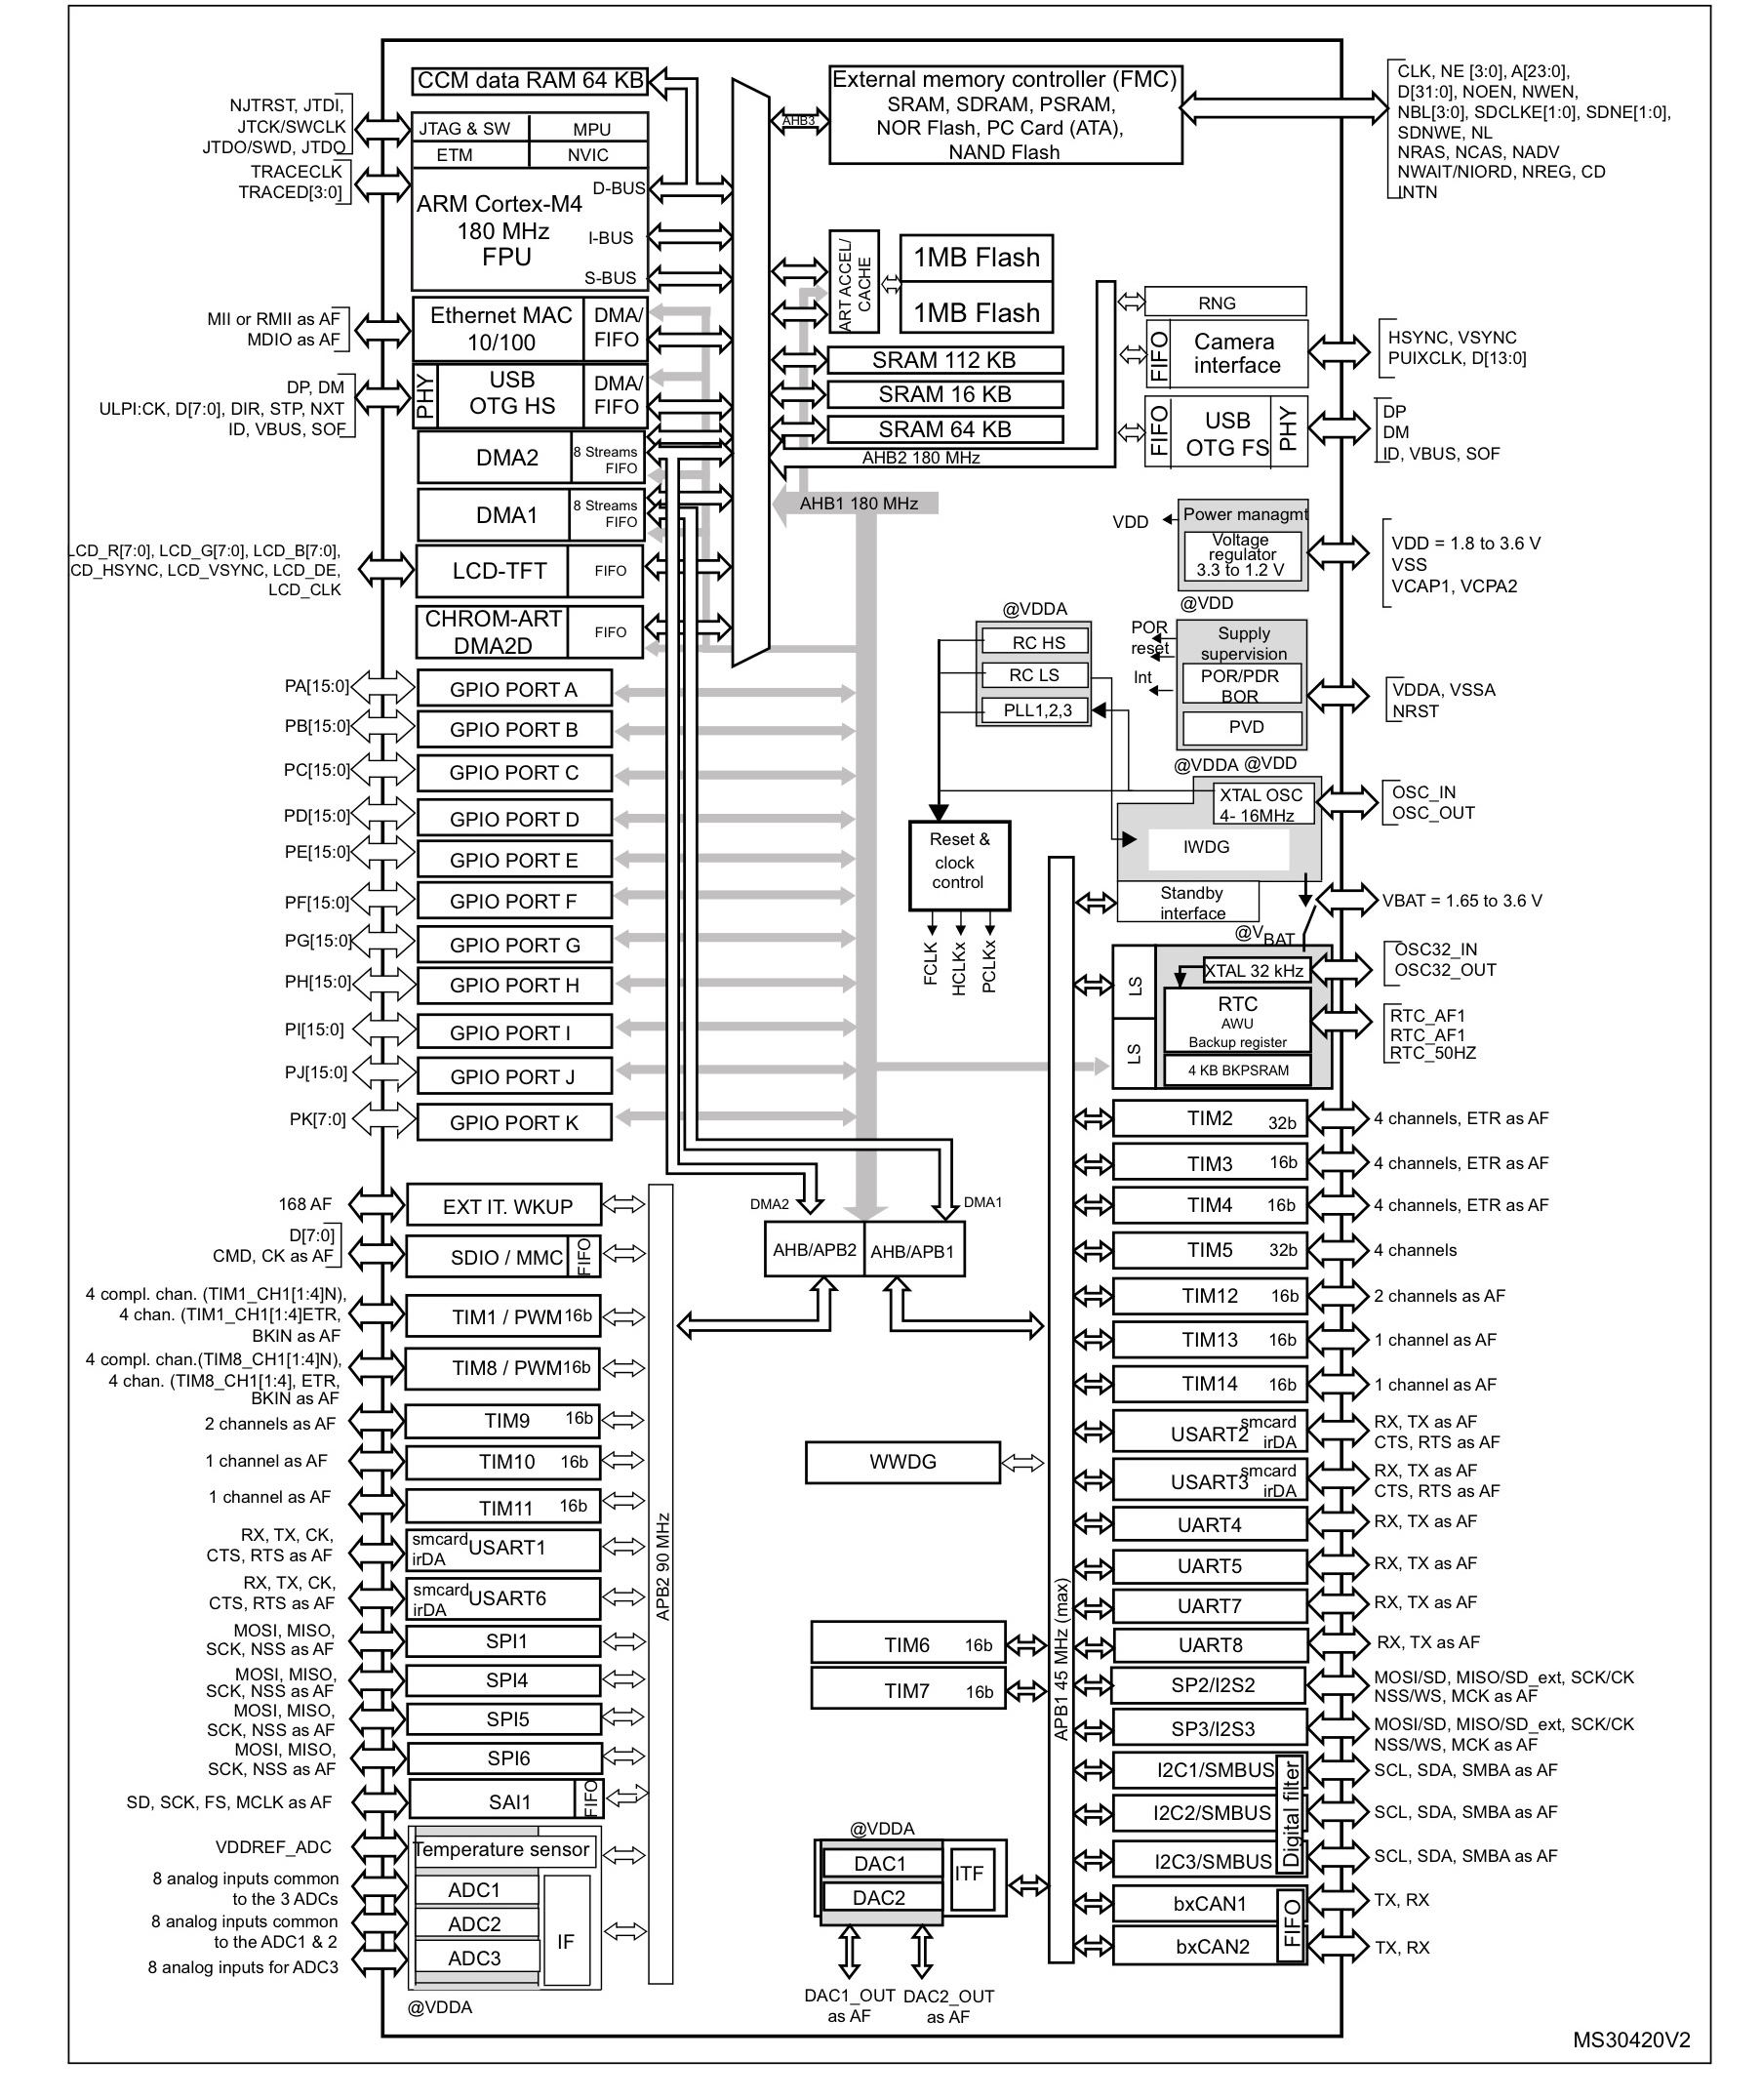
\includegraphics[width=0.8\linewidth]{fotos/diagrama bloque.jpeg}
        \caption{Diagrama de bloques para el STM32F429 \cite{STM2}}
        \label{diag_bloques}
    \end{figure}
    
    
    %diagrama de pines 
    \subsubsection{Diagrama de pines}
    De la misma hoja de datos, se obtienen los diagrama de pines para la sección superior e inferior de la placa que se muestra a continuación: 
        
    \begin{figure}[H]
        \centering
        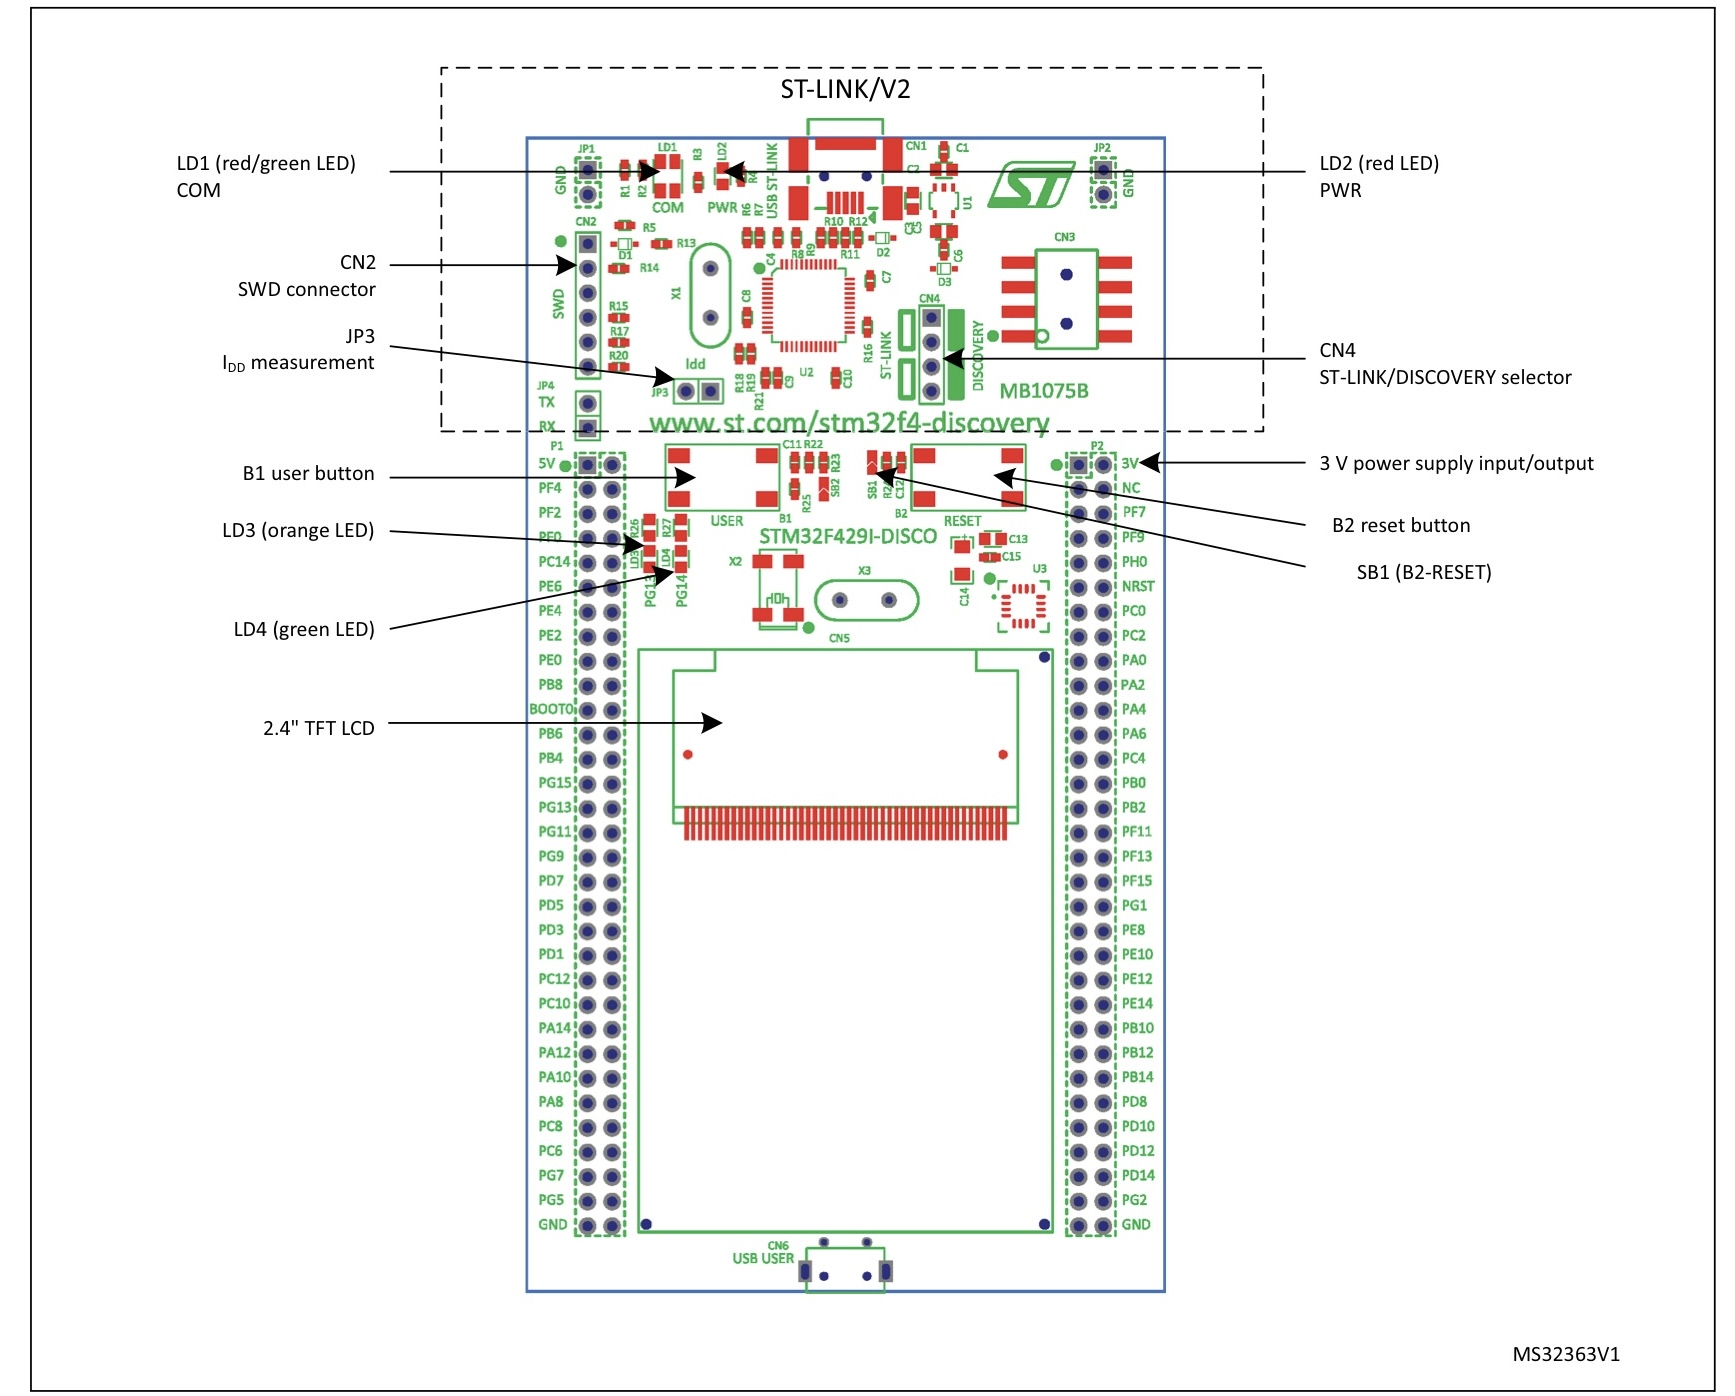
\includegraphics[width=0.8\linewidth]{fotos/pin top.jpeg}
        \caption{Diagrama de pines superior para el STM32F429. \cite{STM2}}
        \label{diag_pines_top}
    \end{figure}

    \begin{figure}[H]
        \centering
        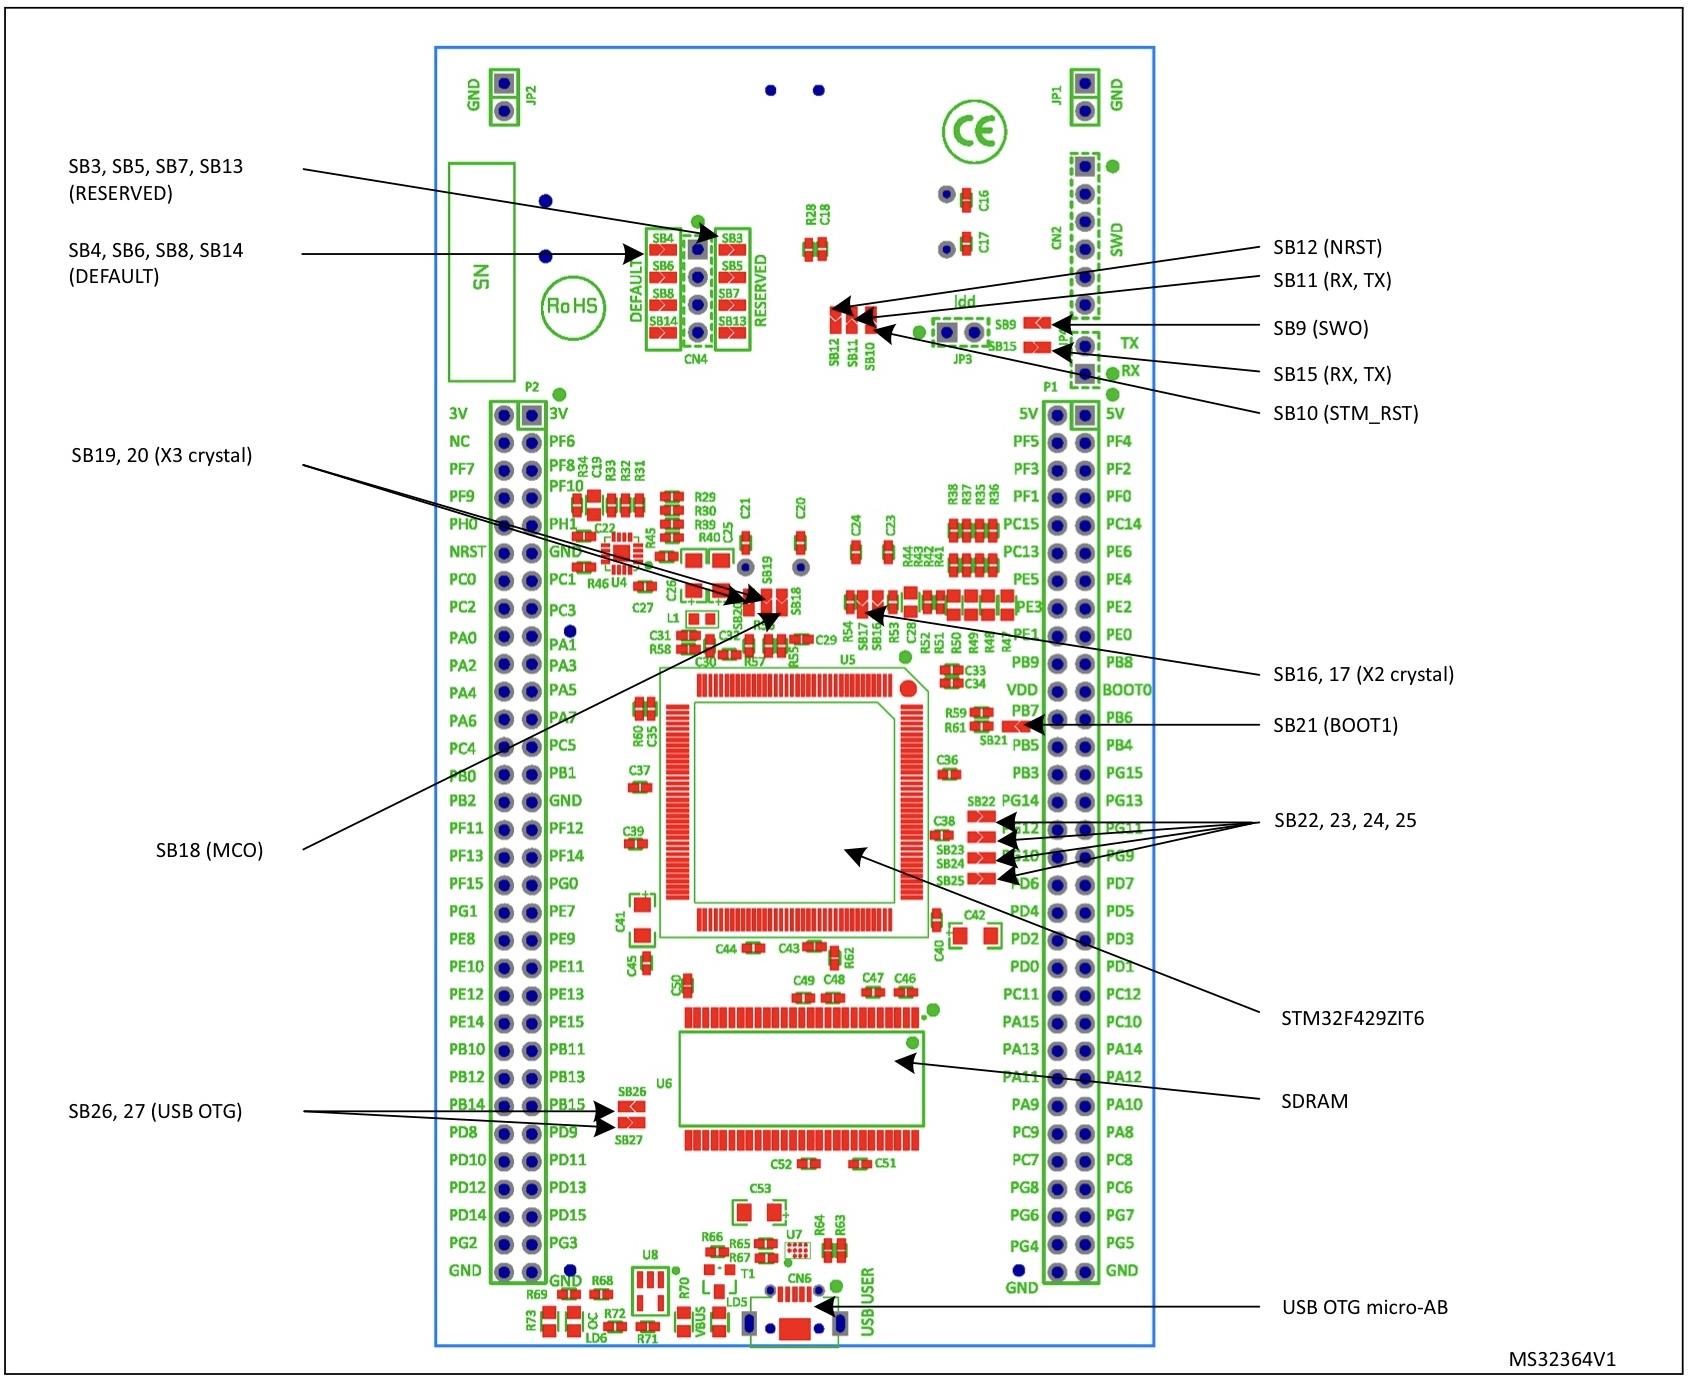
\includegraphics[width=0.8\linewidth]{fotos/pin bottom.jpeg}
        \caption{Diagrama de pines inferior para el STM32F429. \cite{STM2}}
        \label{diag_pines_bottom}
    \end{figure}

    % Giroscopio
\subsubsection{L3GD20}
 Este MCU tiene incorporado el sensor de movimiento L3GD20 de la marca STMicroelectronics, el cual actúa como un giroscopio digital de salida de 3 ejes (x,y,z). \cite{STM} Este sensor es de bajo consumo energético y sensa la velocidad angular de 3 ejes. El sensor provee la medición al mundo externo a través de una interfaz digital ($I^{2}C/SPI$). 

 El dispositivo contiene un conjunto de registros que son utilizados para controlar su comportamiento y para recuperar los datos de la velocidad angular. Cada dirección de registro hace uso de 7 bits, bits que se usan para identificar los registros y para escribir los datos a través de la interfaz serial \cite{sensor}:
 \begin{itemize}
     \item WHO\_AM\_I: para identificar el dispositivo
     \item CTRL\_REG1: Habilita los ejes (x,y,z), selecciona el ancho de banda y energiza al sensor.
     \item CTRL\_REG2: Configura el modo del filtro paso alto.
     \item CTRL\_REG4: para configuraciones adicionales como la escala de sensibilidad
 \end{itemize}

    % Pantalla
    \subsubsection{TFT LCD}

    Asimismo, también contiene una pantalla llamada TFT LCD, siglas en inglés cuya traducción al español sería, una pantalla de cristal líquido con un transistor de capa o película fina \cite{STM}. 
    
    %caracteristicas electricas
    \subsection{Características eléctricas}
    
    Las especificaciones eléctricas del microcontrolador se encuentran en la hoja de datos, y se detallan en la siguiente figura:
    \begin{figure}[H]
        \centering
        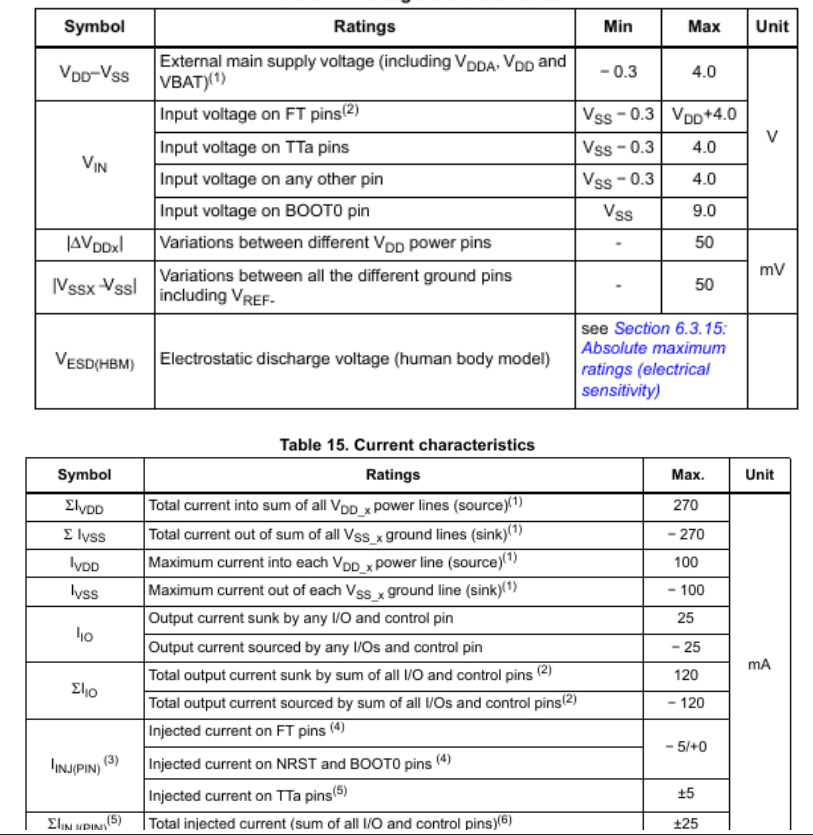
\includegraphics[width=0.5\linewidth]{fotos/caracteristicas electricas.png}
        \caption{Especificaciones eléctricas del STM32F429 \cite{STM3}}
        \label{electrica}
    \end{figure}

%%%%%%%%%%%%%%%%%%%%%%%%%%%%%%%%%%%%%%%%%%%%%%%%%%%%
%%%%%%%%%%%%%%%%%%%%%%%%%%%%%%%%%%%%%%%%%%%%%%%%%%%%

%• Periféricos
\subsection{Periféricos}

%descripción de registros e instrucciones

Cada vez que se mueve la placa, esta va a detectar los cambios en el eje x y z gracias a las lecturas proporcionadas por el giroscopio, y los valores impresos cambian conforme se recibe los datos. El SPI5 es el encargado de inicializar el giroscopio incorporado en la placa stm23. Se realiza la configuración del SPI para operar en modo master, donde se establecen parámetros como la velocidad de reloj (con el baudrate), la polaridad y fase del clock, el modo dúplex completo (para transmisión y recepción simultáneas) y el tamaño de los datos. Para la lectura de los datos del giroscopio, el STM32F429 envía un comando de lectura por medio del SPI, seguido por la dirección del registro del giroscopio que se busca leer, y una vez que ese comando es recibido, el giroscopio responde enviando los datos solicitados de vuelta al MCU. \\

Con respecto a la configuración de los pines GPIO, a continuación se detallan la función de cada uno:
\begin{itemize}
    \item \textbf{GPIO9} del puerto \textbf{A} para la transmisión TX de datos por el USART1.
    \item \textbf{GPIO1} del puerto \textbf{C}, pin de selección de chip (CS) para la comunicación SPI con el giroscopio. Se pone a bajo para activar el giroscopio antes de enviar comandos o leer datos, y se pone a alto después de completar la transacción.
    \item Puerto \textbf{F} de los \textbf{GPIO7, GPIO8, GPIO9}: comunicación SPI con el giroscopio.
    \item \textbf{GPIO0} puerto \textbf{A}: se utiliza para el botón de entrada, donde lectura de este pin va a definir si la comunicación USART se encuentra habilitada o no.
    \item \textbf{GPIO13} puerto \textbf{G}: para el LED verde que va a indiciar el estado de la comunicación USART.
    \item textbf{GPIO13} puerto \textbf{G}: LED verde que señala el estado de la batería
    \item \textbf{GPIO3} puerto \textbf{A}: para leer el voltaje de la batería a través del ADC.
\end{itemize}


   \begin{figure}[H]
        \centering
        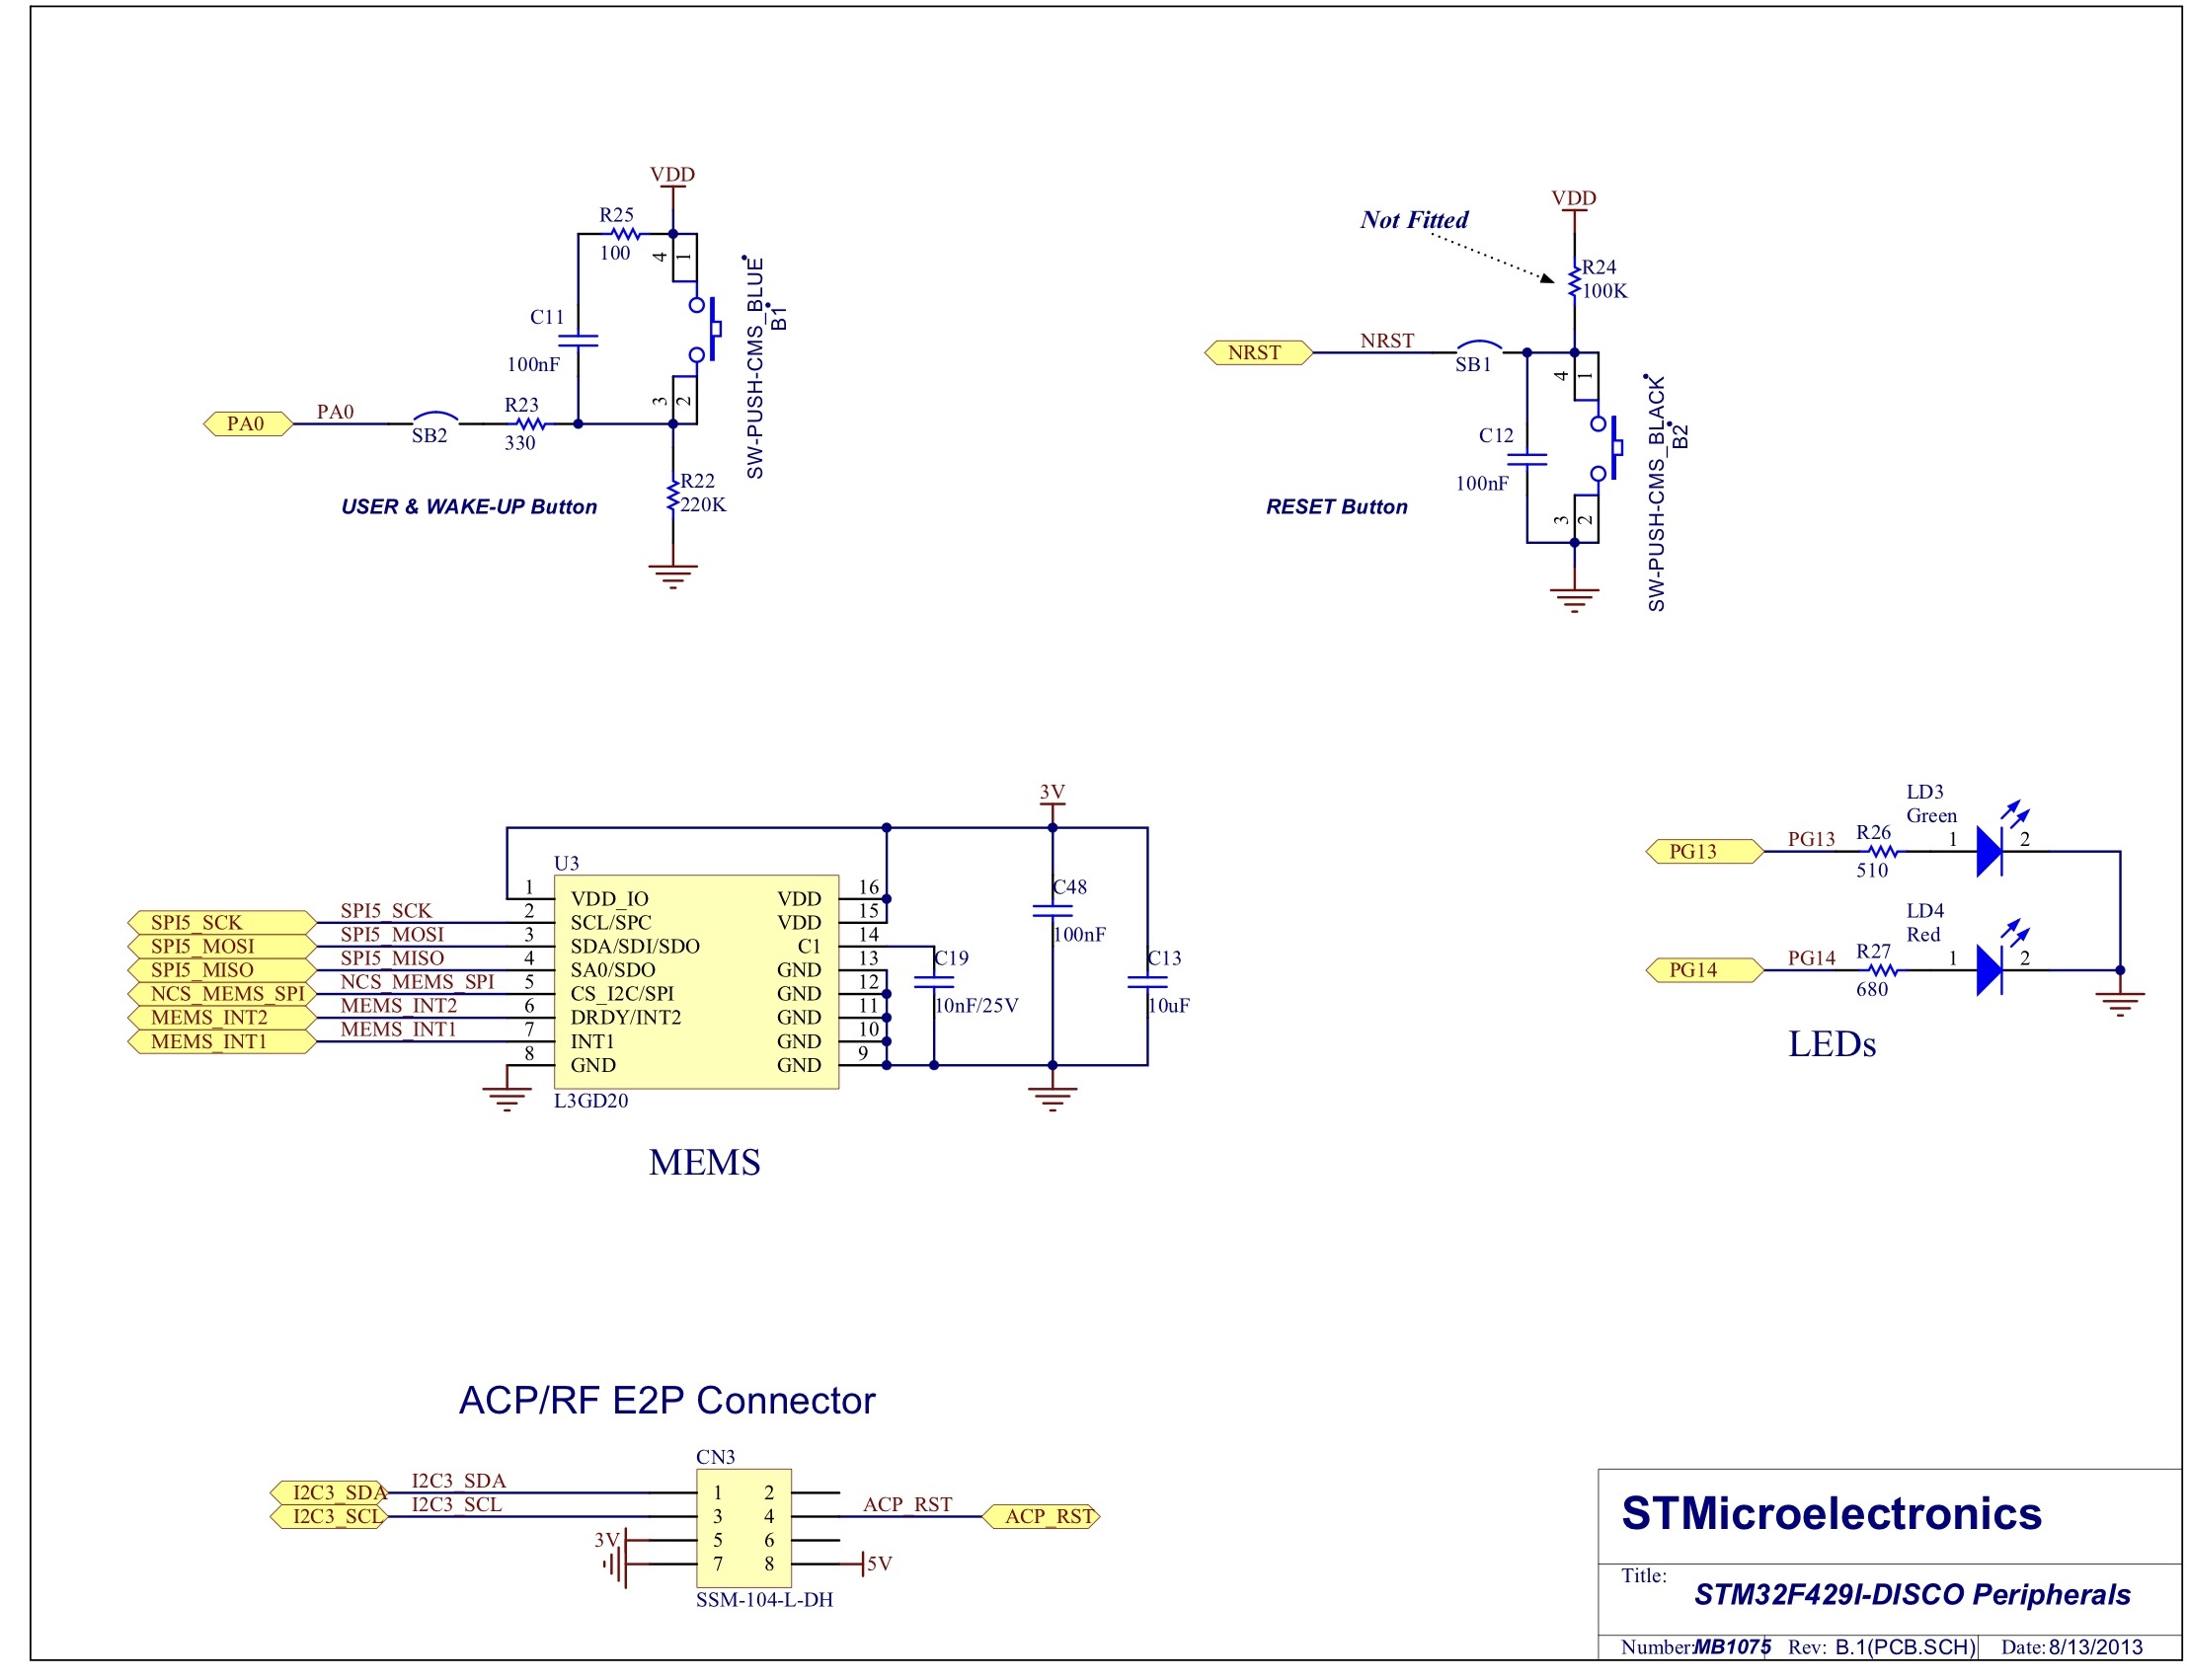
\includegraphics[width=0.65\linewidth]{fotos/perifericos.jpeg}
        \caption{Periféricos del STM32F429}
        \label{peripherals}
    \end{figure}

%%%%%%%%%%%%%%%%%%%%%%%%%%%%%%%%%%%%%%%%%%%%%%%%%%%%
%%%%%%%%%%%%%%%%%%%%%%%%%%%%%%%%%%%%%%%%%%%%%%%%%%%%


%• Lista de componentes y precios
\subsection{Lista de componentes y precios}

\begin{table}[H]
\centering
\begin{tabular}{|l|l|}
\hline
Componente & Precio \\ \hline
Resistencia & ₡100 \\ \hline
Protoboard & ₡2400  \\ \hline
Batería 9V & ₡2300 \\ \hline
\end{tabular}
\caption{Lista de precio para los componentes utilizados}
\label{precios}
\end{table}


%%%%%%%%%%%%%%%%%%%%%%%%%%%%%%%%%%%%%%%%%%%%%%%%%%%%
%%%%%%%%%%%%%%%%%%%%%%%%%%%%%%%%%%%%%%%%%%%%%%%%%%%%

